\documentclass[12pt, twoside, openany]{book}
\linespread{1.25}
\pagestyle{plain}
% --- Packages
% -------------------
\usepackage[a4paper,top=2.5cm,bottom=2.5cm,left=3.5cm,right=2cm]{geometry}
\usepackage[utf8]{inputenc}
\usepackage[T1]{fontenc}
\usepackage{graphicx}
\usepackage{url}

% --- additional packages
\usepackage{epsfig}
\usepackage{epstopdf}
%\usepackage[chapter]{algorithm}
\usepackage{algorithmic}
%\usepackage{listings}
\usepackage{amsmath}
\usepackage{amssymb}
\usepackage{multirow}
\usepackage{booktabs}
\usepackage{color}
\usepackage{setspace}
\usepackage{tabularx}
\usepackage{textcomp}
\usepackage{caption}
\usepackage{natbib}
\usepackage{subcaption}
\usepackage[font=large]{subcaption}
\usepackage{emptypage}
\usepackage{float}
\usepackage[hidelinks,breaklinks]{hyperref}

\usepackage{amsmath}

% -------------------
% --- Definicia zakladnych pojmov
% -------------------
\def\mfrok{2023}
\def\mftitle{An adaptive fuzzy inference in predator-prey pursuit game}
\def\mfthesistype{Master thesis}
\def\mfauthor{Valeriia Danina}
\def\mfskolitel{prof. RNDr. Dušan Guller, PhD.}
\def\mfplacedate{Bratislava, 2023}
\def\mfuniversity{COMENIUS UNIVERSITY IN BRATISLAVA}
\def\mffaculty{FACULTY OF MATHEMATICS PHYSICS AND INFORMATICS}
\def\mfodbor{Applied informatics}
\def\program{Applied informatics}
\def\mfpracovisko{Department of Applied Informatics }
\begin{document}
\frontmatter


% -------------------
% --- Obalka ------
% -------------------
\thispagestyle{empty}

\noindent
\begin{minipage}{\textwidth}
    \begin{center}
        \textbf{\mfuniversity \\
        \mffaculty}
    \end{center}
\end{minipage}

\vfill
\begin{figure}[!hbt]
	\begin{center}
		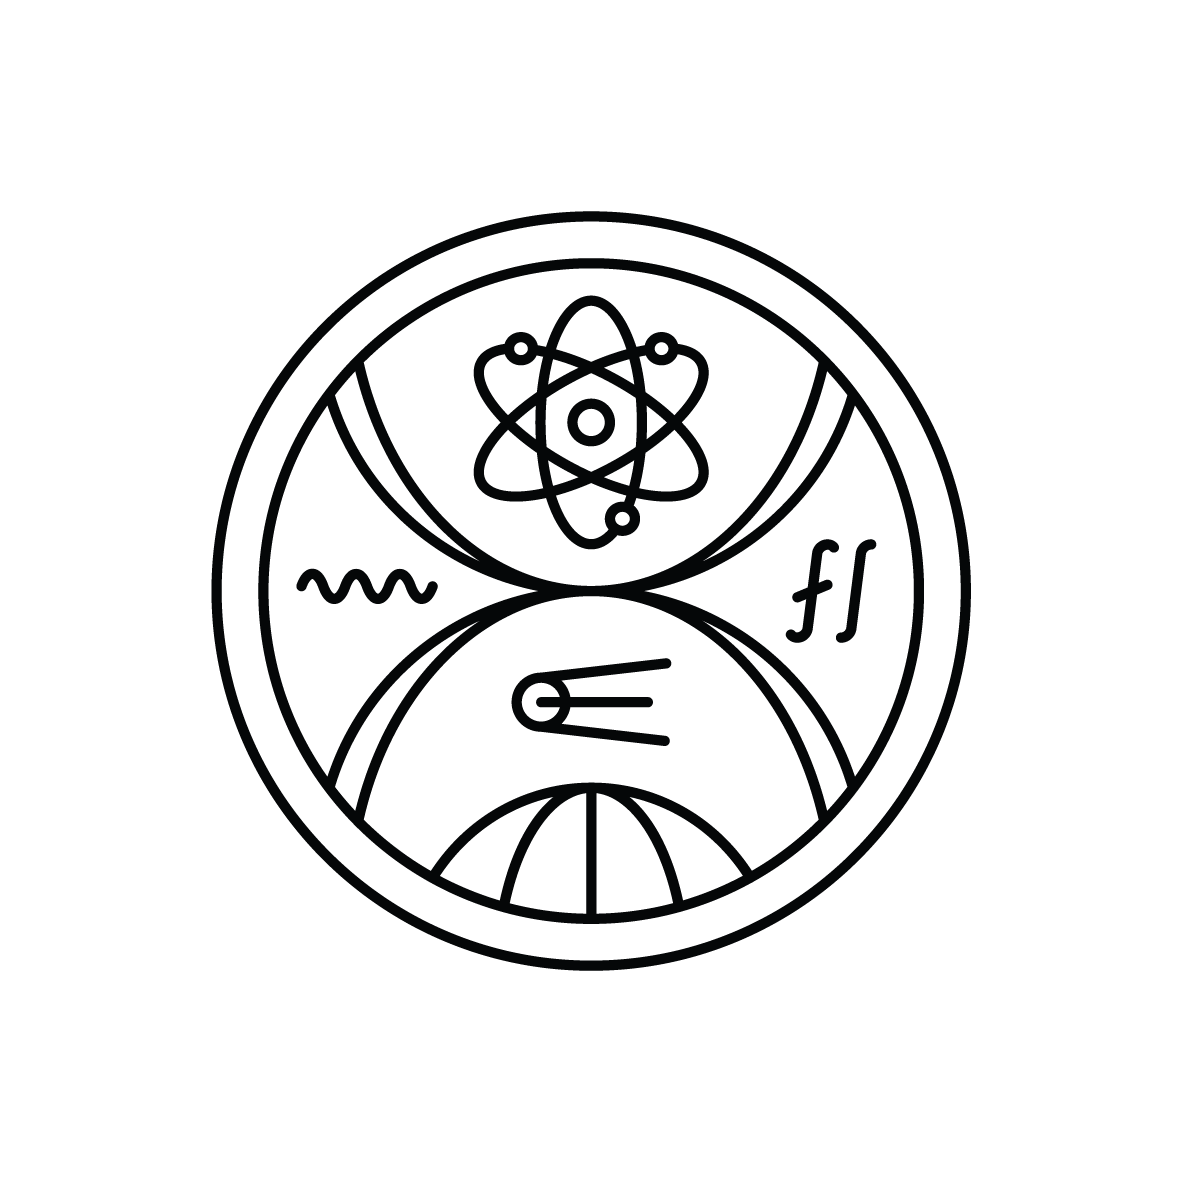
\includegraphics[width=0.4\textwidth]{images/FMFI_logo_BP.png}
		\label{img:logo}
	\end{center}
\end{figure}
\begin{center}
		\textbf{\MakeUppercase{\Large\mftitle}}\\
		\mfthesistype
\end{center}
\vfill
\mfrok \hfill
\mfauthor
%\eject 
\cleardoublepage
% --- koniec obalky ----
% -------------------
% --- Titulný list
% -------------------
\thispagestyle{empty}
\noindent
\begin{minipage}{\textwidth}
    \begin{center}
        \textbf{\mfuniversity \\
        \mffaculty}
    \end{center}
\end{minipage}

\vfill
\begin{figure}[!hbt]
    \begin{center}
        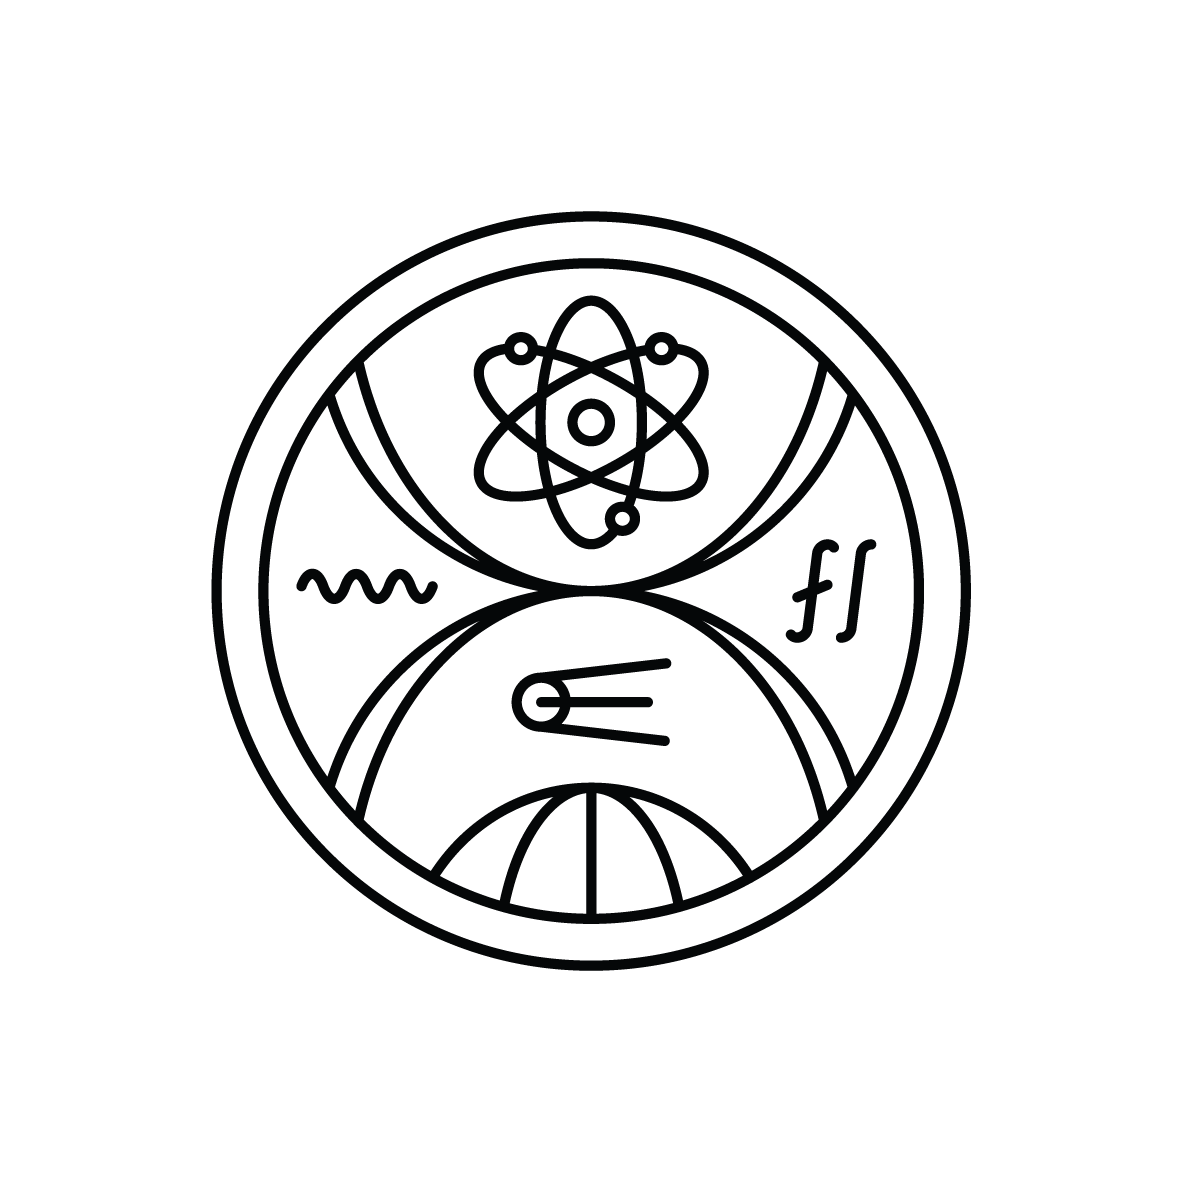
\includegraphics[width=0.4\textwidth]{images/FMFI_logo_BP.png}
        \label{img:logo_dark}
    \end{center}
\end{figure}

\begin{center}
	\textbf{\MakeUppercase{\Large\mftitle}}\\
	\mfthesistype
\end{center}
\vfill


\begin{tabular}{l l}
Study program: & \program \\
Branch of study: & \mfodbor \\
Department: & \mfpracovisko \\
Supervisor: & \mfskolitel \\
\end{tabular}

\vfill
\noindent
\mfplacedate \hfill
\mfauthor
%\eject 
\cleardoublepage
% --- Koniec titulnej strany
% -------------------
% --- Zadanie z AIS
% -------------------
% v tlačenej verzii s podpismi zainteresovaných osôb.
% v elektronickej verzii sa zverejňuje zadanie bez podpisov
% v pracach v naglictine anglicke aj slovenske zadanie

\newpage 
\thispagestyle{empty}
\hspace{-2cm}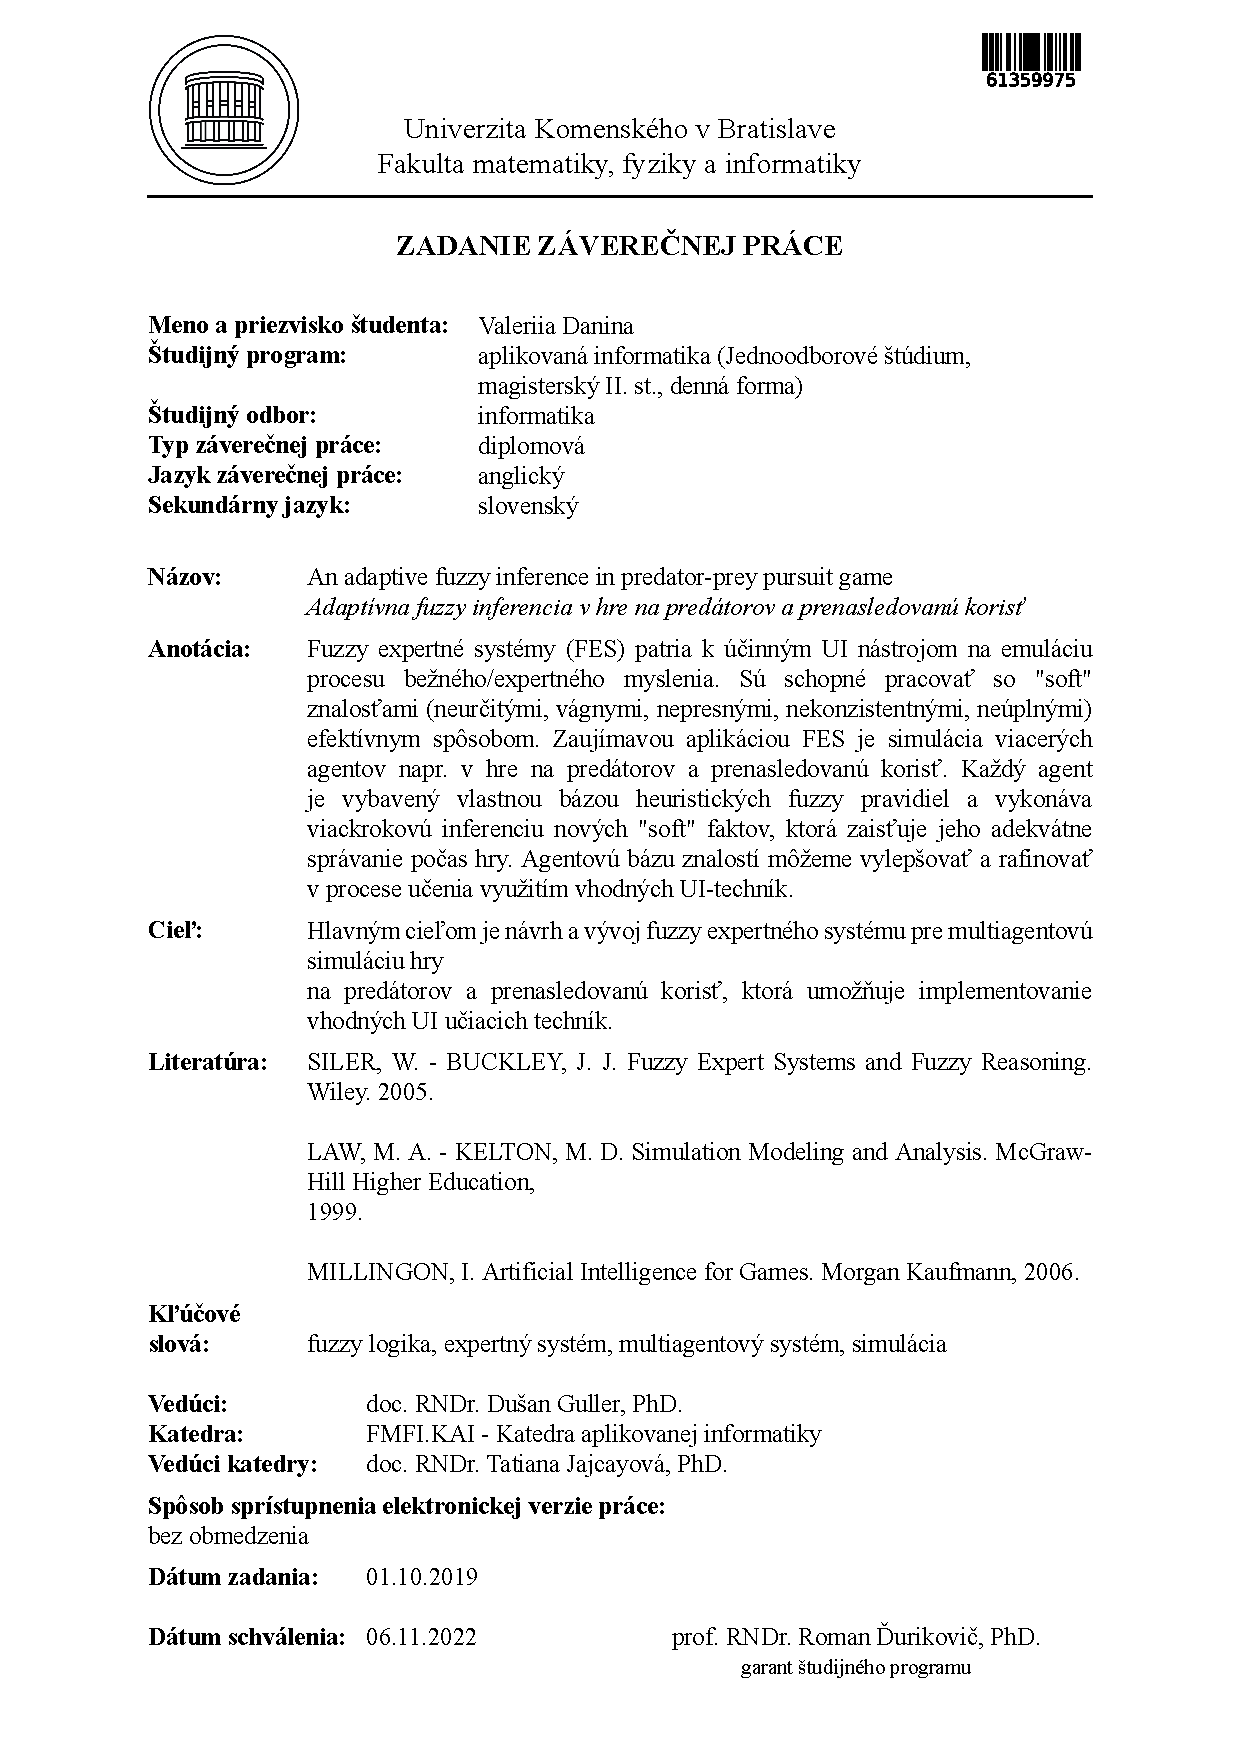
\includegraphics[page=1,width=1.1\textwidth]{zadaniePrace.PDF}

\newpage 
\thispagestyle{empty}
\hspace{-2cm}\includegraphics[page=2,width=1.1\textwidth]{zadaniePrace.PDF}

% --- Koniec zadania

% -------------------
% --- Prehlásenie
% -------------------

{~}\vspace{12cm}

\noindent
\begin{minipage}{0.25\textwidth}~\end{minipage}
\thispagestyle{empty}
\begin{minipage}{0.75\textwidth}
I hereby declare that I have written this thesis by myself, only with help of referenced literature, under the careful supervision of my thesis advisor.
\newline \newline
\end{minipage}
\vfill
~ \hfill {\hbox to 6cm{\dotfill}} \\
\mfplacedate \hfill \mfauthor
\vfill\eject \cleardoublepage
% --- koniec prehlasenia

% -------------------
% --- Abstrakty
% -------------------
\newpage 
\thispagestyle{empty}
\chapter*{Abstract}\label{chap:abstract_en}



\paragraph*{Keywords: fuzzy logic, expert system, multiagent system, simulation}  


\newpage 
\thispagestyle{empty}
\chapter*{Abstrakt}\label{chap:abstract_sk}
\input{abstrakt}

\paragraph*{Kľúčové slová: fuzzy logika, expertný systém, multiagentový systém, simulácia}


% --- koniec abstraktov---
% --- koniec abstraktov


% -------------------
% --- Obsah
% -------------------
\newpage 
\tableofcontents

% ---  Koniec Obsahu



\mainmatter

\chapter{Introduction to fuzzy modeling}
Fuzzy modeling is a special branch of mathematical modeling that has two goals:
(i) to construct models based on information that can be given not only in numbers
but also, imprecisely, usually in a form of expressions of natural language; (ii) to
construct models with less computational demands, which are more robust, that is,
little sensitive to changes in the input data.

In comparison with classical models, the fuzzy ones are closer to human way of
thinking. For example, when processing images, classical methods work with single
pixels. People, however, do not see pixels but larger and usually imprecisely delineated parts of the image. This is the main reason why it is so difficult to develop
methods that are as powerful as the human eye. It happens quite often that some objective measure says that a given image is good, but the human eye sees it differently and
says “no”.

Fuzzy modeling is a group of special mathematical methods that make it possible to
include in the model imprecise or vaguely formulated expert information that is often
characterized using natural language. The developed models (we call them fuzzy
models) are very successful because they provide solution in situations when traditional mathematical models fail—either due to their non-adequacy, or due to their
inability to utilize the full available information.

Note that the idea to include imprecise information in our models contradicts to what has always been required: as high precision as possible. However, there is a good reason for doing it, we face a variance between relevance and precision. The so-called principle of incompatibility \cite{zadeh} says the following:

As a complexity of a system increases, our ability to make absolute, precise, and significant statements about the system's behavior reduces. At some moment, there will be a trade-off between precision and relevance. Increase in precision can be gained only through decrease in relevance; increase in relevance can be gained only through decrease in precision.

But at the same time, we argue that full precision is only our illusion and is not achievable, even in principle. Otherwise, we could obtain the same result independently on the chosen precision. But this is, in general, impossible. 

The attempt to utilize the imprecise information in mathematical models led to the
development of fuzzy modeling techniques. Recall that mathematical models manipulate with variables. In traditional models, values of the considered variable are taken
from some set of numbers called a universe. Traditional mathematical models manipulate directly with its elements. In a fuzzy model, however, variables may represent
fuzzy subsets of the universe. Hence, fuzzy models require partitioning of the universe into parts, for which it is specific that they need not be precisely formed and
can overlap \cite{NOPEDV16}.

The most important tool in fuzzy modeling are fuzzy IF-THEN rules. These are
special expressions, which characterize relations among parts of two or more universes. For example, let us consider an electric boiler and two universes: values
of electric current (A) and temperature  (\(^\circ\)  C ). Then the following is a typical fuzzy IF-THEN rule: IF electric current is very strong, THEN temperature is high.

Benefits of a fuzzy (inference) systems.
\begin{itemize}
    \item This system can handle all kinds of input, even if the information is not exact, unclear or has background noise.
\item Making Fuzzy Logic Systems is simple and easy to understand.
\item Fuzzy logic uses math ideas called set theory, and its reasoning is easy to understand.
\item This helps solve difficult problems in many areas of life really well because it works like how a person thinks and makes choices.
\item The computer rules can be explained using only a small amount of information, so it doesn't need much space to remember.
\end{itemize}

Not so good things about fuzzy (inference) system.
\begin{itemize}
    \item Lots of scientists have ideas to fix a problem with fuzzy logic, which might make things unclear. We don't have a set way to solve a problem using fuzzy logic.
    \item It's usually hard or impossible to prove what makes it unique because we don't always have a mathematical explanation of how we do it.
\item Fuzzy logic uses both exact and inexact information, which can lead to less accuracy.
\end{itemize}

Applications
\begin{itemize}
    \item This thing helps spacecraft and satellites stay at the right height in outer space. People use it in the aerospace industry.
\item This thing helps control how fast cars go and how traffic moves.
\item It helps big companies make better decisions and assess individuals.
\item This thing can be used in the chemical industry to control the pH, help with drying things, and with a process called chemical distillation.
\item Fuzzy logic is a type of math that helps computers understand human language and do smart things. It's very useful in AI.
\item Fuzzy logic is often used in modern control systems, like expert systems.
\item Fuzzy Logic works like a person's decision-making process, but faster, and it is often used with Neural Networks. To make data more meaningful, we combine it and create partial truths using Fuzzy sets.
\end{itemize}

It should be emphasized that robustness is a typical feature not only of fuzzy
control, but also of applications of fuzzy modeling in general. For example, when
applying fuzzy modeling methods to character recognition, we need only few patterns, while in classical solutions, we need hundreds of them. 




%%%%%% does not need to cite

% articles about streaks
% https://cds.cern.ch/record/1707548/files/978-1-4939-0629-1_BookBackMatter.pdf
% https://conference.sdo.esoc.esa.int/proceedings/neosst1/paper/444/NEOSST1-paper444.pdf
% https://www.aanda.org/articles/aa/full_html/2020/12/aa37765-20/aa37765-20.html
% https://reader.elsevier.com/reader/sd/pii/S0094576521001211?token=93F8903DF4BF28EC64C9DE8B86B59D6C71136A835A32EB40977BA9A729EB5DAFCCF2437D4B81A5717C58E2BC46B52704&originRegion=eu-west-1&originCreation=20210804182521

% articles about astronomical imagining
% https://link.springer.com/chapter/10.1007/978-3-319-21969-1_37
% https://subarutelescope.org/staff/guyon/15teaching.web/00AstrOptics.web/AstrOpt_01fund.pdf

% articles about ccd artifacts
% https://arxiv.org/pdf/1601.07182.pdf
% https://mwcraig.github.io/ccd-as-book/01-00-Understanding-an-astronomical-CCD-image.html

% articles about noises
% https://hamamatsu.magnet.fsu.edu/articles/ccdsnr.html
% https://www.mssl.ucl.ac.uk/www_detector/ccdgroup/optheory/darkcurrent.html
% https://camera.hamamatsu.com/jp/en/technical_guides/calculating_snr/index.html








\chapter{Analysis of problematic} \label{chap:astronomicaldata}

% nejaky obkec o tom ze data sa ziskavaju cez teleskopy a tie maju CCD chipy a ze snimky su vo formate FITS. a potom ze v tejto casti prejdeme rozne features ktore sa na snimkach nachadzaju, scenare a defekty a ako tieto nezaduce data odstranujeme
% FITS frames
% AGO data

Many of the most interesting dynamics in nature have to do with interactions between organisms. These interactions are often subtle, indirect, and difficult to detect. Interactions in which one organism consumes all or part of another. This includes predator-prey, herbivore-plant, and parasite-host interactions. These linkages are the prime movers of energy through food chains. They are an important factor in the ecology of populations, determining the mortality of prey and the birth of new predators.

A connected system of predator and prey should cycle, according to mathematical models and common sense: predators grow in number when prey is abundant, predation reduces prey populations to low levels, predator numbers fall, and prey populations rise indefinitely. The Lotka-Volterra Model is one such model that mimics predator-prey interactions.

\section{Classical version of predator-prey game}


The classical predator-prey model is a mathematical model used to study the dynamics of populations in a predator-prey ecosystem. The model typically consists of a set of ordinary differential equations that describe the change in the population of two species, such as predators and prey, over time.

The model considers the rate of change in the prey population as a function of their own birth and death rates, and the rate of predation by the predators. Similarly, the rate of change in the predator population is a function of their own birth and death rates, and the rate of prey consumed.

The model assumes that the populations of both species are continuously growing or declining depending on the balance of birth and death rates, and the interaction between the two species. In particular, the prey population grows when there are few predators and declines when there are many, and the predator population declines when there is little prey and grows when there is plenty.

This model helps to understand the underlying mechanisms driving the fluctuations in populations of both species, and can be used to make predictions about future population dynamics based on changes in environmental conditions or other factors.

The Lotka-Volterra equations describe an ecological predator-prey (or parasite-host) model which assumes that, for a set of fixed positive constants \(a\) (the growth rate of prey), \(b\) (the rate at which predators destroy prey), \(r\) (the death rate of predators), and \(c\) (the rate at which predators increase by consuming prey). The following conditions will be held for our computer simulation model.

Let the prey population at time t be given by \(y_1(t)\), and the predator population by \(y_2(t)\). Assume that, in the absence of predators, the prey will grow exponentially according to \(y_1' = a \ y_1\) for a certain \(a > 0\). We also assume that the death rate of the prey due to interaction is proportional to \(y_1(t) \ y_2(t)\), with a positive proportionality constant. So:
\(\\ y_1' (t) = a\ y_1(t) - b\ y_1(t)\ y_2(t)   \)

Without prey, predators will die exponentially according to \(y_2'(t)=-r\ y_2\ dt\) for a certain \(r>0\). Their birth strongly depends on both population sizes, so we finally find for a certain \(c>0\):
\( \\ y_2'(t) = -r\ y_2(t) + c\ y_1(t)\ y_2(t)  \)

These equations lead to the following system of differential equations:  

$$ \left\{
\begin{array}{lr}
y_1'(t) = a\ y_1(t) - b\ y_1(t)\ y_2(t)\\
y_2'(t) = -r\ y_2(t) + c\ y_1(t)\ y_2(t)
\end{array}
\right. $$
\newline
 
We see that both \(( e^{at}, 0)\) and \((0, e^{-ct} )\) are solutions of \((y_1(t), y_2(t))\). From this system, we find that for every solution we must have 
\(y_1' (\frac{r}{y_1} - c) +y_2' (\frac{a}{y_2} - b) = 0 \).

Integrating both sides give us: 
\[r\ log\ y_1(t) – c\ y_1(t) + a\ log\ y_2(t)\ –\ b\ y_2(t) = constant. \]

The Lotka-Volterra equations are a pair of first-order, non-linear, differential equations that describe the dynamics of biological systems in which two species interact. The earliest predator-prey model based on sound mathematical principles forms the basis of many models used today in the analysis of population dynamics, the original form has problems \cite{cpp1}.

The game is usually represented by a payoff matrix, where each entry represents the payoffs (or utilities) to the predator and prey given their current strategies. The strategies in this game correspond to the population sizes of the predator and prey, and the payoffs are determined by the underlying population dynamics described by the predator-prey model.

For example, suppose the prey population grows at a rate proportional to its size and the predator population grows at a rate proportional to the number of prey consumed. Then, the payoffs to the predator and prey can be represented as follows:


Predator Payoff = \((a - b) * P - c * Q\),

Prey Payoff = \(d * Q - e * P\),


where \(P\) and \(Q\) are the population sizes of the predator and prey, respectively, \(a, b, c, d,\) and \(e\) are positive constants representing the growth and death rates of the populations, and the terms \((a - b) * P\) and \(d * Q\) represent the intrinsic growth rates of the populations. The terms \(-c * Q\) and \(-e * P\) represent the costs of predation and being preyed upon, respectively.

This game has a unique Nash equilibrium, which is a state where neither player has an incentive to change its strategy, given the strategies of the other player. At the Nash equilibrium, the population sizes of both species are stable and remain constant over time.

The classical predator-prey game provides a framework for analyzing the interplay between the populations of predators and prey in an ecosystem, and can be used to understand the factors that influence the stability and persistence of both species.

\section{Adaptive neuro‑fuzzy inference system (ANFIS)}
An adaptive network is a multi-layer feedforward network in which each node performs a particular
function (node function) on incoming signals as well as a set of parameters pertaining to this node. The nature
of the node functions may vary from node to node, and the choice of each node function depends on the overall
input-output function which the adaptive network is required to carry out.

ANFIS represent Sugeno Takagi fuzzy models and uses a hybrid learning algorithm. For simplicity, we assume the fuzzy inference system under consideration has two inputs x and y and one output z. Suppose that the rule base contains two fuzzy if-then rules of Takagi and Sugeno’s type:


Rule 1: If \(x\) is \(A1\) and \(y\) is \(B1\), then \(f1 = p1\ x + q1\ y + r1\);

Rule 2: If \(x\) is \(A2\) and \(y\) is \(B2\), then \(f2 = p2\ x + q2\ y + r\).

\section{Small modifications of predator-prey game} \label{sec:features}
There are several ways in which the classical predator-prey game can be modified to better reflect the complexities of real-world ecosystems. Some common modifications include:

1. Adding multiple prey species: In many ecosystems, predators consume multiple prey species, and the interactions between these species can have important consequences for population dynamics. To reflect this, the predator-prey game can be extended to include multiple prey species, each with its own growth and death rates, and the predator's payoffs can depend on the populations of all the prey species.

2. Incorporating resource competition: In many ecosystems, prey species compete for limited resources, and this competition can affect both their growth and death rates. To incorporate this competition, the prey-prey interaction can be modeled as a separate game, and the payoffs to the prey species can depend on the populations of other prey species.

3. Allowing for adaptive behavior: In real-world ecosystems, the populations of both predators and prey can evolve, leading to changes in their behavior and interactions. To reflect this, the predator-prey game can be extended to allow for evolutionary dynamics, where the populations of both species can evolve to better adapt to their environment.

4. Incorporating habitat destruction: Human activities, such as deforestation and urbanization, can significantly alter the habitats of both predators and prey, and this can affect their population dynamics. To reflect this, the predator-prey game can be extended to include a third player, representing the habitat, and the payoffs to the predator and prey can depend on the state of the habitat.

These modifications can provide a more accurate representation of real-world ecosystems, and help to shed light on the complex interactions between predators, prey, and their environment. However, they also introduce additional complexities and can make the analysis of the predator-prey game more challenging.

\section{Current overview of fuzzy modeling predator-prey game} \label{sec:scenarios}

Scientists use predator-prey models to study how animals that hunt (predators) and animals that are hunted (prey) interact in a certain environment. Fuzzy modeling is a way to study complicated things using fuzzy logic.

In a fuzzy game, the population dynamics of predators and prey are modeled using fuzzy logic. Fuzzy logic helps us understand better how predators and prey relate to each other. It does this by considering the fact that ecological systems are often uncertain and imprecise.

You can use a fuzzy inference system to model a game where a fuzzy predator chases a fuzzy prey. It has three parts: making things fuzzy, figuring out what to do, and making things clear again. Fuzzification is when we turn simple information like how many people live somewhere or things in the environment into fuzzy groups. Inference means using fuzzy rules to make predictions about how predators and prey populations will change. Defuzzification means changing the unclear results back into clear data.

Fuzzy modeling has been applied to predator-prey games in various ways to understand the behavior of the agents and to develop optimal strategies for managing populations in real-world scenarios. Here are some current overviews of fuzzy modeling predator-prey games:

Fuzzy logic-based predator-prey models: These models use fuzzy logic to develop rules for the agents' behavior based on their characteristics and the environment. The rules are defined using linguistic terms and fuzzy sets that represent the degree of membership of an agent in a particular category. These models have been used to simulate different scenarios and to evaluate the effectiveness of different strategies for managing predator and prey populations.

Fuzzy game theory-based predator-prey models: These models use fuzzy logic and game theory to analyze the behavior of the agents in predator-prey games. The models are based on the assumption that both predators and prey have incomplete information about the behavior of the other agents and are uncertain about the outcome of their actions. The models use fuzzy logic to represent the uncertainty and game theory to analyze the interactions between the agents.

Fuzzy reinforcement learning-based predator-prey models: These models use fuzzy logic and reinforcement learning to develop optimal strategies for the agents in predator-prey games. The models use fuzzy logic to represent the state of the environment and the actions of the agents and use reinforcement learning algorithms to learn the best actions to take in different situations. These models have been used to develop effective strategies for managing predator and prey populations in real-world scenarios.

Overall, fuzzy modeling can provide a more comprehensive and accurate representation of the complex dynamics between predators and prey in ecological systems. It can also be used to explore different scenarios and predict the outcomes of different management strategies.

\section{A review of some recent modifications} \label{sec:defects}


There have been several recent modifications of fuzzy modeling predator-prey games to improve their accuracy and effectiveness. Here are some examples:

Hybrid fuzzy systems: Some researchers have combined fuzzy logic with other techniques such as neural networks or genetic algorithms to create hybrid fuzzy systems. These systems can improve the accuracy and robustness of the models by combining the strengths of different techniques. 

Multi-objective optimization: Some recent models have used multi-objective optimization to develop strategies that balance multiple objectives, such as maximizing the predator's success rate while minimizing the impact on the prey population. These models can provide more realistic and sustainable solutions to managing predator and prey populations. 

Multi objective optimization problem is the process of simultaneously optimizing two or more
conflicting objectives subject to certain constraints. Such problems can be found in various
fields: product and process design, finance, aircraft design, the oil and gas industry, automobile
design, or wherever optimal decisions need to be taken in the presence of trade‐offs between
two or more conflicting objectives. Genetic algorithms are a particular class of evolutionary
algorithms that use techniques inspired by evolutionary biology such as inheritance, mutation,
selection, and crossover and is the most commonly used search techniques in computing to find
exact or approximate solutions to such optimization and search problems.


In real world problems, parameters of a process are never precisely fixed to a definite value.
Transients, noise, measurement errors, Instrument’s least count etc makes it even more difficult
to know their exact value at any time stamp. Even if externally regulated, parameters have some
variability in their values. This variability has been continuously ignored by using
mean/approximated/fixed value of the parameters, thus losing the precious information about
the variability in the final optimized solution.

Dynamic models: Some researchers have developed dynamic fuzzy models that can adapt to changes in the environment and the behavior of the agents. These models can simulate more realistic scenarios and can be used to study the long-term effects of different management strategies.

Agent-based models: Some recent models have used agent-based modeling to simulate the behavior of individual agents in predator-prey games. These models can provide a more detailed understanding of the behavior of the agents and can be used to develop more precise management strategies.

Fuzzy decision-making: Some researchers have used fuzzy decision-making to develop strategies for managing predator and prey populations. These models use fuzzy logic to evaluate the effectiveness of different strategies and to select the best course of action based on the current state of the environment and the behavior of the agents.

Overall, these recent modifications of fuzzy modeling predator-prey games have improved the accuracy and effectiveness of the models and have provided new insights into the dynamics of predator-prey interactions. Further developments in fuzzy modeling techniques are likely to continue to improve our understanding of these complex systems and to provide more effective management strategies for predator and prey populations.




% -------------------
% --- Bibliografia
% -------------------

\backmatter

\nocite{*}
\bibliographystyle{plain}
\bibliography{references}

%---koniec bibliografie


\end{document}